
%%%%%%%%%%%%%%%%%%%%%%%%%%%%%%%%%%%%%%%%%%%%%%%%%%%%%%%%%%%%%%%%%%%%%%%%%%%%%%%
%%%%%%%%%%%%%%%%%%%%%%%%%%%%%%%%%%%%%%%%%%%%%%%%%%%%%%%%%%%%%%%%%%%%%%%%%%%%%%%
%%%%%%%%%%%%%%%%%%%%%%%%%%%%%%%%%%%%%%%%%%%%%%%%%%%%%%%%%%%%%%%%%%%%%%%%%%%%%%%
\section{Results} %-----------------------------------------------------------%
\subsection{Evaluation Platform} %--------------------------------------------%
All results were obtained by either interrogating the daemon directly
to inspect it's state or by running queries against the SOSflow
databases, such as the one in Figure~\ref{example_query}.
%
%\begin{figure}[h]
%  \centering
%  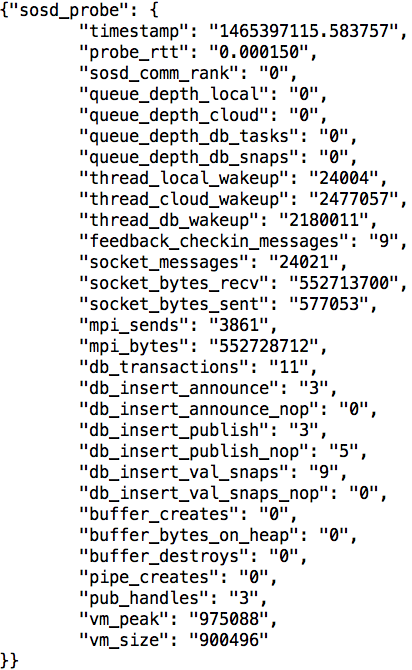
\includegraphics[width=\columnwidth]{images/probe_json_example.png}
%  \caption{JSON Object Returned by SOS's Probe Tool}
%  \label{probe_json}
%\end{figure}
%
%
%


\subsection{Experiment Setup} %-----------------------------------------------%
%
The experiments described here had the following purposes:
\begin{itemize}
\item \textbf{Validation} : Show that the SOSflow model works for a general case
\item \textbf{Exploration} : Observe the overhead and latency of
  SOSflow's current research implementation.
\end {itemize}
%
The SOSflow codes are general purpose and do not feature (or require)
tailoring to the deployment environment.
%
The same SOSflow code base was used for each of the experiments.
%
\subsubsection{Oregon:ACISS} %-------------------------------------------------------%
Tests run on the ACISS platform at the University of Oregon were
deployed with the Torque job scheduler as MPICH2 MPI applications at
scales ranging from 3 to 24 nodes, serving 10 configurable synthetic
data-producing processes per node in all cases.
%
The ACISS battery of runs were tuned as stress tests to make ensure
the daemons could operate under reasonably heavy loads.
%
In the 24-node ACISS experiment (Figure~\ref{aciss_lat_24_agg}),
SOSflow processed 72,000,000 values during a 90 second window
containing three rounds of extremely dense API calls.
%
%
\subsubsection{NERSC:Cori} %--------------------------------------------------%
Real-world use case experiments were conducted on the Cori
supercomputer at The National Energy Research Scientific Computing
Center NERSC.
%
An SOSflow-enabled branch of the Tuning and Analysis Utilities program
(TAUflow) was created as a part of the SOSflow development work.
%
On Cori, TAUflow was used to instrument the Livermore Unstructured
Lagrangian Explicit Shock Hydrodynamics (LULESH) code.
%
During the execution of LULESH, a thread in TAUflow would periodically
awaken and submit all of TAU's observed performance metrics into the
SOSflow system.
%
Power and memory consumption data was collected and stored by SOSflow
for each node and LULESH process.
%
\par
%
During the execution of the workflow, a visualization application was
launched from outside of the job allocation which connected to the
online (in situ) database and was able to query and display a
graph of the metrics that SOSflow had gathered.
%
TODO ---- GRAPH HERE
%
This experiment was run both with and without the presence of SOSflow
(all other settings being equal) in order to validate that ability of
SOSflow to meet the its design goals while being minimally invasive.
%
TODO ---- MORE (ref to graph)
%
%
\subsubsection{LLNL: Catalyst} %----------------------------------------------%
Latency tests were performed on LLNL's Catalyst machine at
various scales up to 128 nodes, with 8 data sources contributing
concurrently on each node in each case.
%
The latency observed at the on-node database at all
scales was not significantly different.
%
The results from the largest 128-node runs are presented here.
%
Results from smaller runs are omitted for space, as they show nothing
new: ``Time in flight'' queue latency at smaller scales linearly
approached the injection latency figures for the on-node database.
%
These tests measured the latency introduced by sweeping across three
different parameters:
\begin{itemize}
\item Count of unique values per publication handle
\item Number of publish operations per loop
\item Delay between calls to the publish API
\end{itemize}
%
Exploring the optimal configuration and utilization of SOSflow is left
to future research effort.
%
TODO ---- INSERT CHARTS (have from ST'16 slides)
%
These initial results are promising, given the research version of SOSflow
being profiled has not benefitted from rigorous optimization work.
%
In the largest runs, across all configurations, the mean latency
observed was ~0.3 seconds (and a maximum of 0.7 seconds) for a value,
and its full complement of metadata and timestamps, to migrate from
one of 1,024 processes to the off-node aggregate data store, passing
through multiple asynchronous queues and messaging systems on 128
nodes.
%
%
\subsubsection{Aggregation Topology}
%%%%%
The current version of SOSflow is configured at launch with a set
number of aggregator databases.
%
The validation tests on ACISS used 3 sosd(db) instances to divide up
the workload, while the TAUflow + LULESH experiments on Cori used a
single aggregator.
%
The parameter sweeps run on the LLNL Catalyst machine were done with
four sosd(db) aggregation targets at 128 nodes.
%
Tests on ACISS and Catalyst were exploring the latency of data
movement through SOSflow, and so both configurations featured
dedicated nodes for sosd(db) aggregators to avoid contention
with other on-node work.
%
The Cori runs captured a real application's behavior, and was primarily
intended to demonstrate the fitness of SOSflow for capturing the
performance of a scientific workflow along with meaningful context.
%
As many instances of aggregators can be spawned as needed in order to
support the quantity of data being injected from a global
perspective.
%
All data sent to SOSflow is tagged with a GUID, shards the global
information space that are split off into a partitions across several
aggregators each can be concatenated after the run concludes without
collision of identities wiping out unique references.
%
%


\subsubsection{Latency} %-----------------------------------------------------%
When a value is published from a client into the SOSflow runtime,
it enters an asynchronous queue scheme for both database injection
and off-node transport to an aggregation target.
%
Latency in this context refers to the amount of time that a value
spends in these queues before becoming available for query by
analytics modules.
%
\par
%
The design choices made for SOSflow do not prioritize the minimization
of latency per se, but focus rather on gracefully handling spikes in
traffic by growing (and then shrinking) the space inside the
asynchronous message queues.
%
Once a value is passed to SOSflow, it is guaranteed to find its
way into the queryable data stores, and there are timestamps attached
to it that capture the moment it was packaged into a publication handle in
the client library, the moment it was published to the daemon, and
even the moment it was finally spooled out into the database.
%
Once it is in the database, it is trivially easy to correlate values
together by the moment of their packing into a publication handle, nomatter
how long the value was sequestered in the asynchronous queues.
%
\par
%
During the ACISS stress-tests, values were being injected into the
SOSflow system faster than they could be spooled from the queues into
the database.  This accounts for the observed saw-tooth pattern of
increasing latency seen in those results.
%
While every value will eventually be processed and injected into the data
store, some values wound up having to wait longer than others as the queue
depth increased.
%
The asynchronous queues have thread-sequential FIFO ordering, but
because the MPI messages are queued up based on their arrival time,
and a batch is handled competely before the next is processed, there
is no real-time interleaving of database value injections, they are
injected in batches.
%
This creates the sawtooth pattern in figures~\ref{aciss_lat_3_agg} and
\ref{aciss_lat_24_agg}, as the latency for values in the batches near
the bottom of the pile of MPI messages consistently increases until
their batch is injected, detailed in
figure~\ref{aciss_lat_3_agg_detail}.
%
%


%%%%%
\begin{figure}[h]
\centering
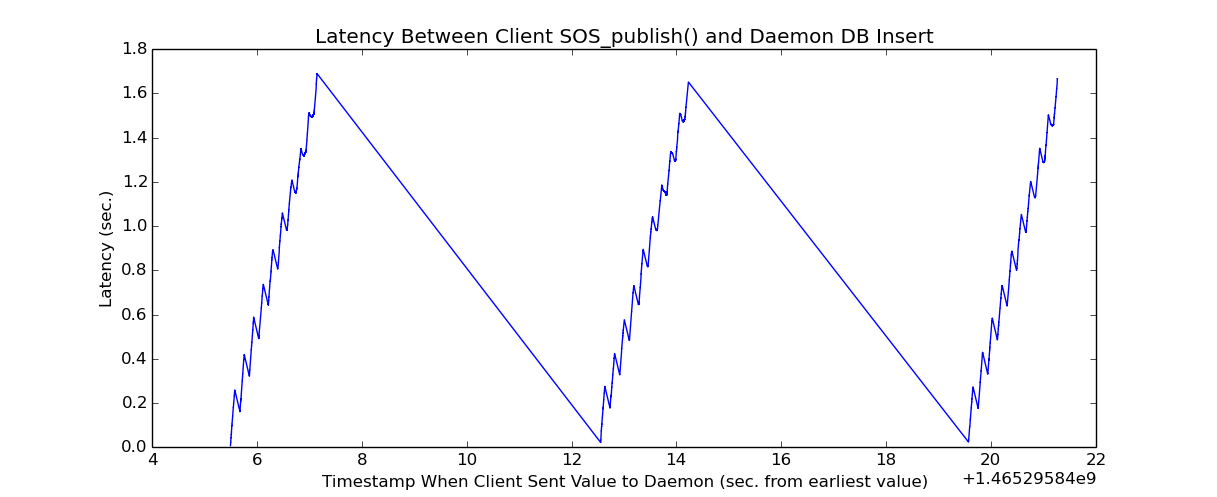
\includegraphics[width=\columnwidth]{images/aciss_latency_3_situ.png}
\caption{In Situ Latency (3 Nodes, 30 Applications)}
\label{aciss_lat_3_situ}
\end{figure}
%%%%%

%%%%%
\begin{figure}[h]
\centering
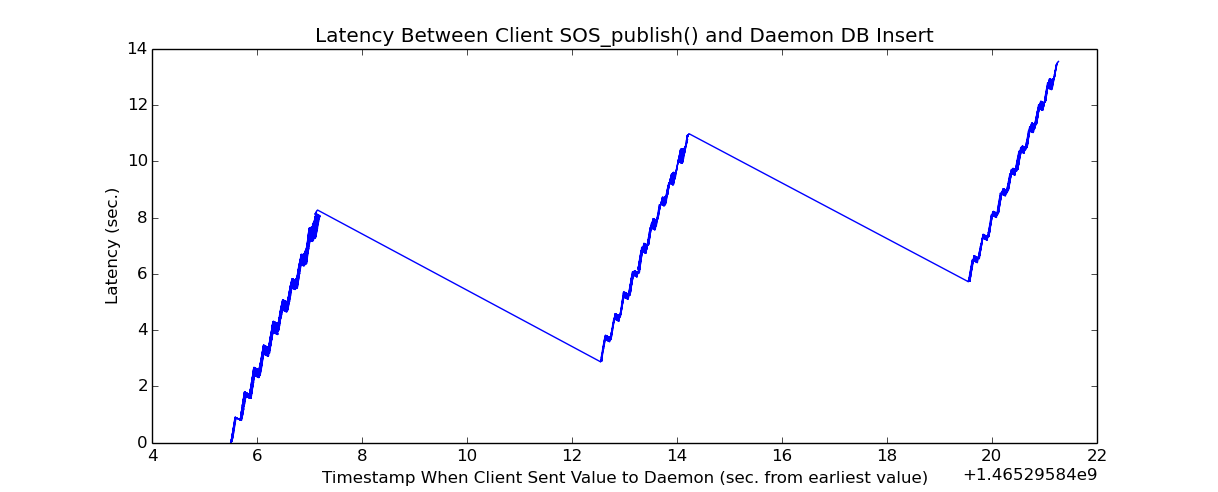
\includegraphics[width=\columnwidth]{images/aciss_latency_3_agg.png}
\caption{Aggregate sosd(db) Latency (3 Nodes, 30 Applications)}
\label{aciss_lat_3_agg}
\end{figure}
%%%%%

%%%%%
\begin{figure}[h]
\centering
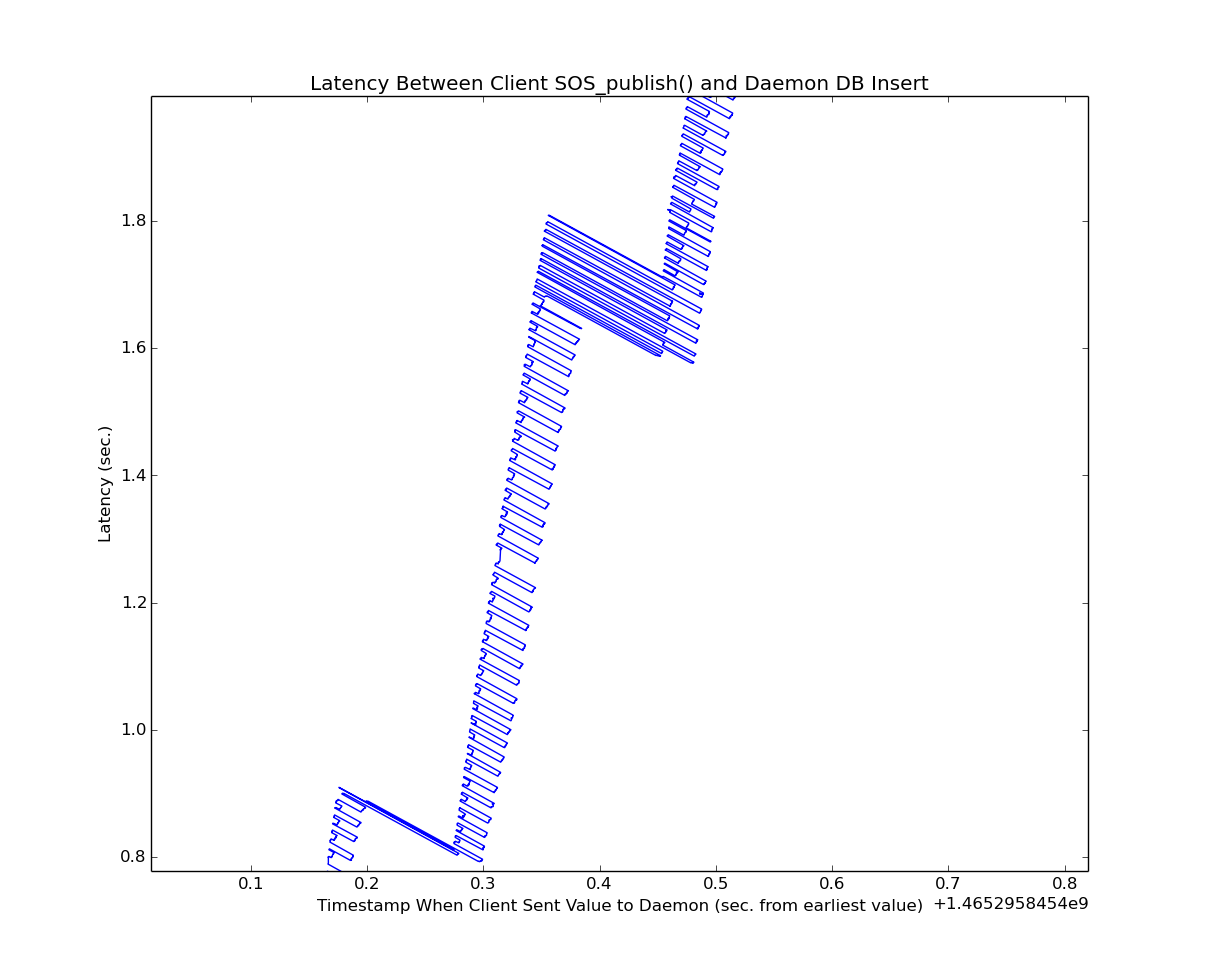
\includegraphics[width=\columnwidth]{images/aciss_latency_3_agg_zm.png}
\caption{Aggregate sosd(db) Detail (3 Nodes, 30 Applications)}
\label{aciss_lat_3_agg_detail}
\end{figure}
%%%%%

%%%%%
\begin{figure}[h]
\centering
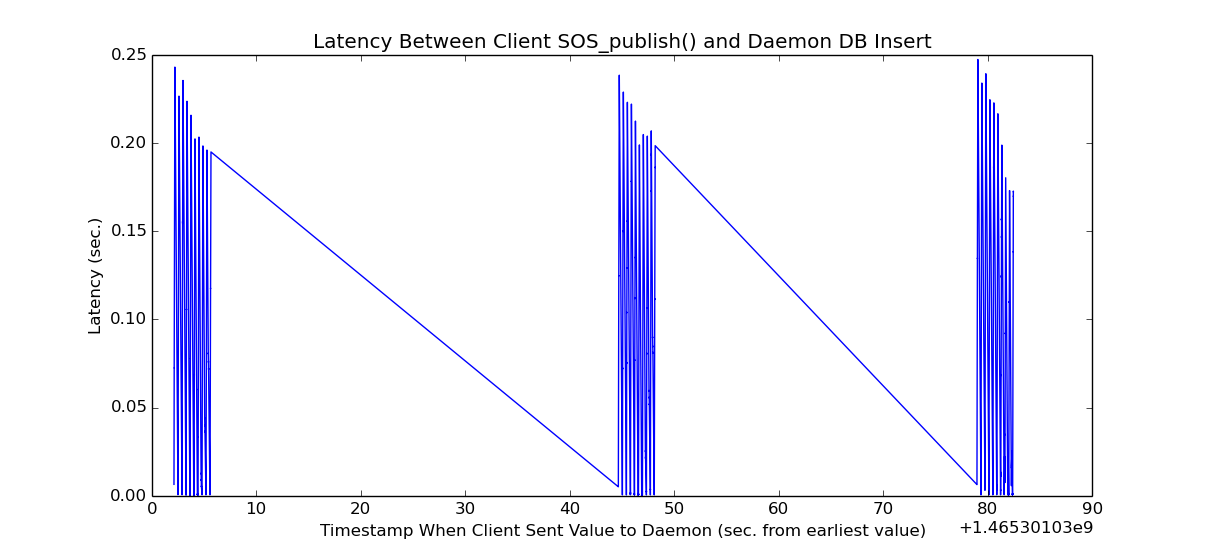
\includegraphics[width=\columnwidth]{images/aciss_latency_24_situ.png}
\caption{In Situ Latency (24 Nodes, 240 Applications)}
\label{aciss_lat_24_situ}
\end{figure}
%%%%%

%%%%%
\begin{figure}[h]
\centering
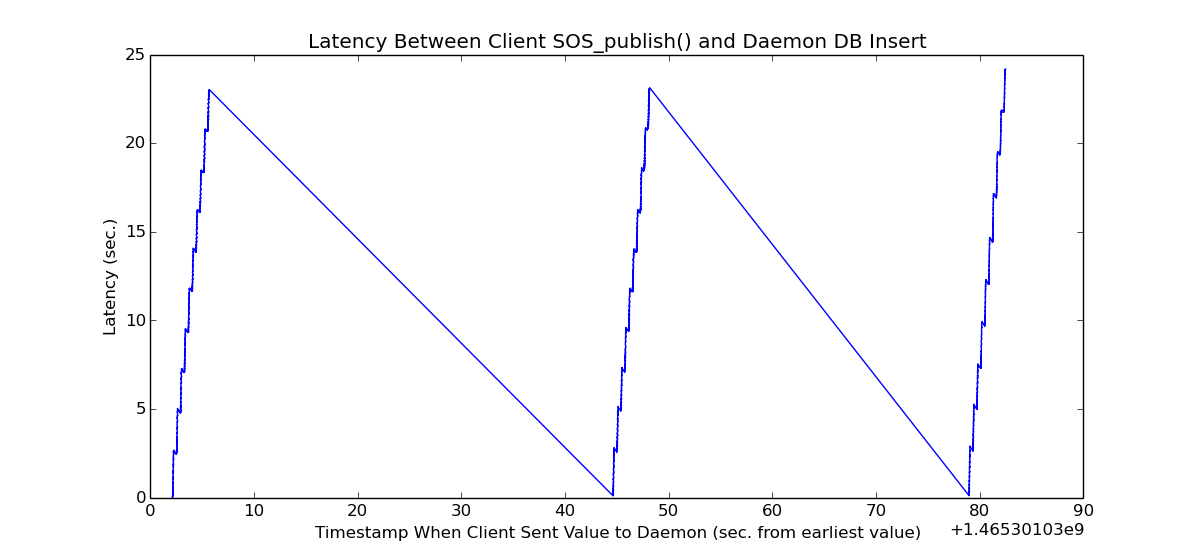
\includegraphics[width=\columnwidth]{images/aciss_latency_24_agg.png}
\caption{Aggregate sosd(db) Latency (24 Nodes, 240 Applications)}
\label{aciss_lat_24_agg}
\end{figure}
%%%%%
%
\par
%



\subsubsection{Time Cost of Publish API} %-----------------------------------%
In situ interactions between libsos rountines and the daemon are
nearly constant time operations regardless of the daemon's workload.
%
Care was taken in the daemon's programming to prioritize rate of message
ingestion over immediacy of message processing so that SOSflow API calls
would not incur onerous delays for application and tool developers.
%
The constancy of message processing speed is shown in
figures~\ref{sock_cost} and \ref{sock_cost_detail}, where the round
trip time (RTT) of a probe message between a client and the daemon
(blue) is projected over a graph of the number of new messages
arriving in a sample window (red).
%
\par
%
This information was fetched by sending 9000+ probe messages over a 15
minute window, with a single sosd(listener) rank processing an average
of 43,423 client messages a minute arriving from four different
processes on an 8-way Xeon node.
%
The messages from SOS clients contained more than 14.7 GB of data,
averaging to 338kB per message.
%
Though there are a few spikes in the probe message RTT visible in
Figure~\ref{sock_cost}, they are likely not related to SOSflow at all,
as Figure~\ref{sock_cost_detail} reveals in detail.
%
The RTT holds steady during low and high volume of traffic from the
other in situ client processes.
%
The mean RTT for the probe messages was 0.003 seconds, and the maximum
RTT was 0.007 seconds.
%%%%%
\begin{figure}[h]
\centering
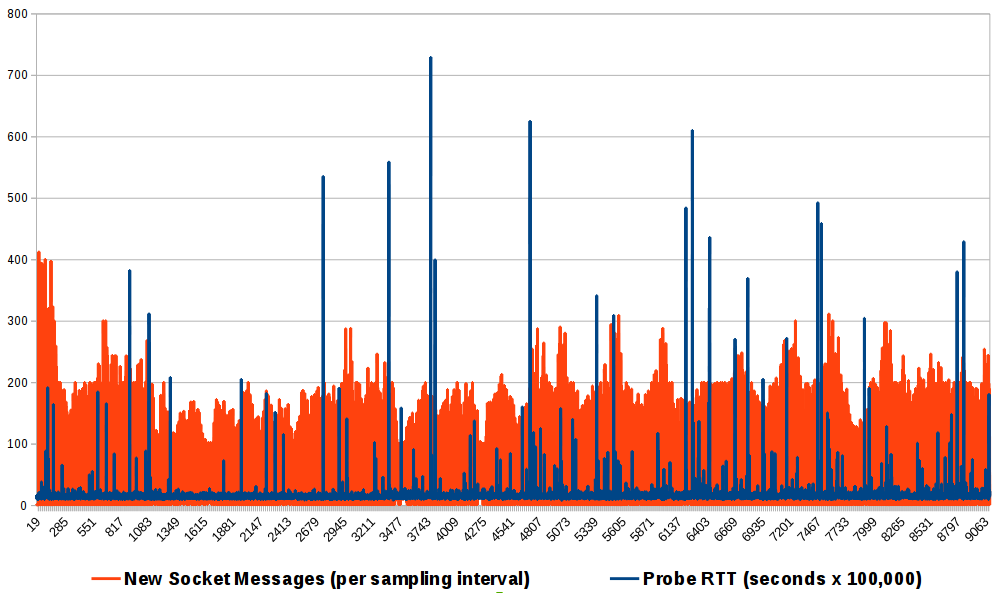
\includegraphics[width=\columnwidth]{images/icebox_api_cost_when_slam.png}
\caption{SOSflow Socket Communication Cost (~0.003sec Mean)}
\label{sock_cost}
\end{figure}
%%%%%

%%%%%
\begin{figure}[h]
\centering
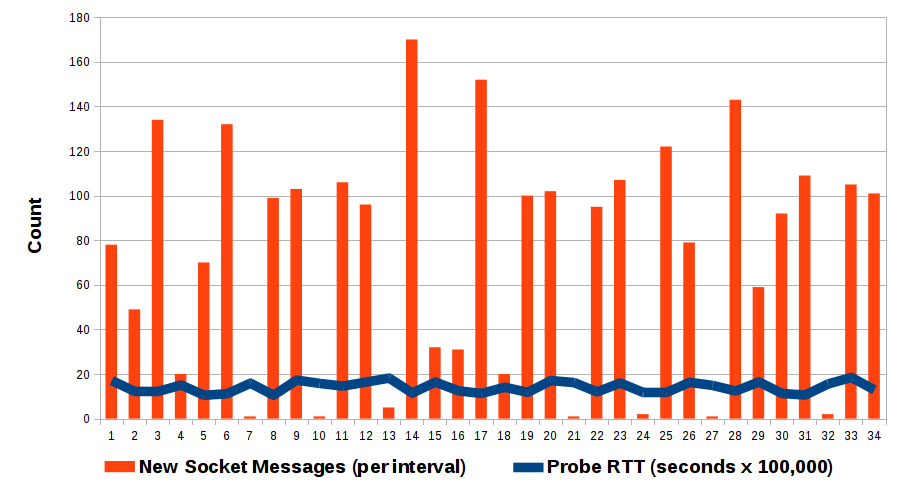
\includegraphics[width=\columnwidth]{images/icebox_api_cost_zoom.png}
\caption{SOSflow Socket Communication Cost, Detail}
\label{sock_cost_detail}
\end{figure}
%%%%%
%
\par
%
These results are promising, because they represent a worst-case
scenario for API calls: Unlike the SOSflow API calls for publishing
data, the probe message used to interrogate the daemon for message
count are relatively slow, as the daemon has to service the request by
packaging up a large struct of its internal statistics to send back to
the client, where normally a simple ACK message is returned.
%
%


\subsection{Discussion} %-----------------------------------------------------%
%
Many of the behavioral characteristics of SOSflow are the product of
its internal parameters and the configuration of its runtime
deployment, rather than products of its data model and algorithms.
%
The exploration of optimal settings in that combined parameter space
is left for future work: For now the effort was made to select
reasonable default SOSflow configuration parameters and
typical/non-priviledged cluster queues and topologies.
%
Because of the general novelty of the architecture, the results
presented here could be considered the \textit{performance baseline}
for SOSflow to improve on as the research line matures.
%
\par
%
TODO ---- MORE (conclusion needs some heft)



%%%
%%%  EOF
%%%
